% algo.tex
%% \section{Output-sensitive Enumeration of Maximal Repeats in a String}
\section{Enumeration of Maximal Repeats}
\label{sec:algo}
%%%% 
In this section, we present our $O(e_R)$-time algorithm scheme $\MREnum$ (\textit{top-down search with the suffix array}) for enumerating all distinct maximal repeats of a string $S$,  based on $\SA, \ISA$, and $\LCP$ with the RMQ structure of a string $S$ using $O(n)$ words of space. The time complexity is upper bounded by a parameter $e_R = e_R(S)$, namely, the number of right-extensions, which is one of the fundamental measures of repetitiveness of strings, and satisfies $|\MR(S)| \le e_R(S) \le n$, and can be logarithmic in $n$ for highly-repetitive strings. Hence, the proposed algorithm can be faster than the previous algorithm with $\Theta(n)$ time complexity for such classes of strings. 

%%%% 
\subsection{Maximal repeats}
%%%%
Maximal repeats of a string is a fundamental concepts in discovery of unusual words, and introduced as follows.  
A \textit{repeat} of $S$ is any substring $u \in \Sigma^+$ that occurs at least twice in $S$, that is, $u \in \Fac(S)$.
Let $u \in \Sigma+$ be any factor of $\hat S$. Since $\#, \daller \not\in \Sigma$, we see $u \in \Fac(S)$, namely, $u$ is contained in the content $S$.

\begin{definition}[maximal repeat]\rm 
A string $u \in \Sigma+$ is a \textit{maximal repeat} of $S$ if it satisfies the following conditions: 
\begin{enumerate*}[(1)]
\item $u$ is a factor of $S$, i.e., $u \in \Fac(S)$;  
\item there exist two start positions $p, q \in \Spos[S](u)\;(p\not= q)$ of $u$ such that
  \begin{enumerate*}[(i)]
  \item $u$ is \textit{left-branching} meaning that the preceding characters are mutually different, i.e., $S[p-1] \not= S[q-1]$, and
  \item $u$ is \textit{right-branching} meaning that the following characters are mutually different, i.e., $S[p+|u|] \not= S[q+|u|]$. 
  \end{enumerate*}
\end{enumerate*}
\end{definition}

In what follows, $\MR(S)$ denotes the set of all maximal repeats of a string $S$. By definition, any $w$ in $\MR(S)$ correctly occurs at least twice in $S$. 
For later use, we define the \textit{set of left characters} $\LSigma(u) \subseteq \Sigma\cup\set{\#}$ (resp.~\textit{right characters} $\RSigma[](u) \subseteq \Sigma\cup\set{\daller}$) of a factor $u \in \Fac(S)$ to be the sets of all characters $S[p-1] \in \hat\Sigma$ (resp.~$S[p+|u|] \in \hat\Sigma$) preceding (resp.~following) all positions $p\in \Spos(u)$ of $u$ in $\hat S$.
If it is clear from context, we write $\LSigma[](u)$ and $\RSigma[](u)$ by omitting subscript $\hat S$. 
Using this notation, we can redefine a maximal repeat of $S$ to be any nonempty string $u \in \Fac(S)$ with $|\LSigma(u)| \ge 2$ and $|\RSigma(u)| \ge 2$.



%% %%%%%%%%%%%%%%%%%
%% {
%%   \setlength{\interspacetitleruled}{0pt}%
%%   \setlength{\algotitleheightrule}{0pt}%  
%%   \begin{algorithm}[h]
%%   %% \caption{Top-down MR-enumeration algorithm with SA}\label{algo:maxrep:tdfw}
%%   \textbf{Procedure} \MREnum$(\tau_0 = ([L_0..R_0], \ell_0))$:\\
%%   %%\KwGiven{}
%%   %% \KwIn{The triple $\tau_0 = (L_0, R_0, \ell_0)$ for a right-branching substring $X$ of a string.}
%%   %% \KwOut{}
%%   \Begin{
%%       \textbf{output} $\tau_0$
%%       \Comment*{A maximal repeat is found}
%%       \For %(\CM{})
%%            {child $\tau = ([L..R], \ell)$ of the parent $([L_0..R_0], \ell_0)$}{
%%           \Comment{It is ensured that $R - L \ge 1$ and $\tau$ is right-branching}
%%           Decide if $\tau$ is left-branching by $SA, ISA$, and $S$ (\cref{lem:leftmaximal:character})\; 
%%           \If {$\tau$ is left-branching}{          
%%             \MREnum$(\tau)$\; 
%%           }
%%         }
%%   }
%%   \end{algorithm}
%% }  
%% %%%%%%%%%%%%%%%%%

%% \subsection{Search strategy}
%%% algo.tex
\subsection{Outline of the algorithm}
\label{sec:algo:tdsa}

%%%%
\begin{algorithm}[t]
  \caption{A basic algorithm that, given a string $S[1..n]$ of length $n$ over alphabet $\Sigma = \set{0, \dots, \sigma-1}$, enumerates all maximal repeats of $S$ within the set $\MR(S)\cap \Theta$ that satisfy a monotone constraint $\Theta$ on $\MRW(S)$. Examples of monontone constraints are
    $\Theta_\idrm{maxlen} = \Sigma^{\le \ell}$ and 
    $\Theta_\idrm{minfreq} = \sete{ u \in \Sigma^*\mid \Occ(u) \ge s }$ for integers $\ell, s\ge 0$.
}\label{fig:example:mrep:main}
\KwNotes{$S$ must satisfies $|\Sigma(S)| \ge 2$; Otherwise, start the procedure with as $root$ the triple for the shortest maximal repeat $\rext{\eps}$ in $S$.
}
\textbf{procedure} $\MREnum(\pair{i..j, \ell}, \Theta, Words)$\;
\Begin{
    Preprocess $\SA, \ISA, \LCP$ from a string $S$\;
    \While (\comblk{Runtime}) {a new request $\Theta$ is given by a user}{
      $Words \gets \emptyset$; 
      $root \gets \pair{1..n, 0}$\; 
      $Words \gets \MRRec(\pair{1..n, 0}, \Theta, Words)$\;
      Output $Words$\; 
    }
  }
\end{algorithm}

\begin{algorithm}[t]
  \caption{A subprocedure $\MRRec$ for enumerating
    the set $\MR(S)$ of all maximal reepeats of the string $S$ prefixed by the word $u := \getfactor(i..j, \ell)$. 
    %% all maximal repeats.
    %% See Algorithm~\ref{fig:example:mrep:main}For  input and output.
}\label{fig:example:mrep:sub}
%%%\medskip
%%  
  %% \KwInput{
  %%   A rich representation $\pair{i..j, \ell}$ for a factor of $S$,
  %%   and a set $Words$ of rich representations over $\pair{\SA, S}$. 
  %% }
  \KwInput{
    A triple $\pair{i..j, \ell} \in \RREP$,
    a monotone constraint $\Theta \subseteq \Sigma^*$, and 
    a set $Words \subseteq \RREP$. 
  }
  %% \KwOutput{
  %%   the set $\MR(S)$ of all maximal reepeats of the string $S$ prefixed by the word $u := \getfactor(i..j, \ell)$. 
  %% }
  \textbf{procedure} \MRRec$(\pair{i..j, \ell}, \Theta, Words)$\;
  \Begin{
      %\textbf{output} $(i..j, \ell)$
      \If{$u := \getfactor(i..j, \ell) \not\in \Theta$}{
        \Return $Words$\; 
      }
      $Words.\append(\pair{i..j, \ell})$
      \Comment*{A maximal repeat is found}
      $Children \gets \emptyset$\; 
      $Children \gets \GenChildren(i..j, \ell, Children)$\Comment*{See \cref{lem:genchildren}}
      \label{line:recmr:for:begin}
      \For {each child $(c, \pair{i_c..j_c, \ell_c}) \in Children$}{
             \Comment{Postcondition:
               %% $|i_c..j_c|\ge 2$ and
               $c \in \LSigma(\getfactor(i..j, \ell))$ and 
               the factor $u_c = \getfactor(i_c..j_c, \ell_c)$
               is a repeat with $|\LSigma(u_c)| \ge 2$.                
             }
             %% \Comment{Postcondition: $|i_c..j_c|\ge 2$ and the triple is right-branching}
          \If (\comblk{See \cref{lem:leftmaximal:character}}) {$\isLeftBranching(i_c..j_c, \ell_c)$}{          
            $Words \gets \MRRec(\pair{i_c..j_c, \ell_c}, \Theta, Words)$\;
            \label{line:recmr:for:end}
          } %% if 
       } %% for 
       \Return $Words$\; 
    }
\end{algorithm}

%%\KwGiven{}
  %% \KwIn{The triple $\tau_0 = (L_0, R_0, \ell_0)$ for a right-branching substring $X$ of a string.}
  %% \KwOut{}
  %%%%%%%%%%%%%%%%%



We show our main procedure $\MREnum$ of our algorithm in Algorithm~\ref{fig:example:mrep:main} and its recursive subprocedure $\MRRec$ in Algorithm~\ref{fig:example:mrep:sub}. 

A basic idea of $\MREnum$ is the use of \textit{top-down search} using the forward search for right-extensions based on the \textit{suffix array}, unlike the backward search for right-extensions adopted by \TDBW.
This enables the sound and early pruning of hopeless right-extensions that never become left-branching ones.
%% 
Now, we define the parent-child relation over triples related to the suffix tree of $S$ as follows. For triples $\tau_0 = ([L_0..R_0], \ell_0)$ and $\tau = ([L..R], \ell)$ defining strings $U$ and $W$, $\tau$ is called the \textit{$b$-child} of $\tau_0$ if $W = Ub$ for some character $b \in \Sigma$, called a \textit{branching character}. The ancestors and descendants of $\tau$ are defined in the standard manner.
%%We have. 

\begin{lemma}\label{lem:prune:leftbranch}
Suppose that a triple $\pi$ is an ancestor of a triple $\tau$. If the substring defined by $\tau$ is left-branching, the substring defined by $\tau$ is also left-branching. 
\end{lemma}

Recall that a repeat is maximal if and only if it is both left- and right-maximal in $S$. Lemma~\cref{lem:prune:leftbranch} says that the set $\MR(S)$ occupies the \textit{upper connected region} of the suffix tree of $S$. For instance, we see in \cref{fig:fwdstree} that $\MR(S)$ occupies the node sets $\set{1,6,15,9}$. 
%% In other words, if a triple $\tau$ is not left-branching, then any of its ancestor is also not left-branching.
This implies the next rule.

\begin{itemize}\item[]
\quad\textsc{Pruning rule}: {Every non-left-branching triple is pruned.}
\end{itemize}


The following lemma is a slight modification of Narisawa \textit{et al.}~\cite[Lemma~10]{narisawa2007efficient}, which gives how to implement the procedure $\isLeftBranching(i..j, \ell)$ that, given a triple $\tau = \pair{i..j, \ell}$, decides whether the factor $\getfactor(\tau)$ is left-branching in an $S$. 
 

%% For testing the left-branching property, we use the following lemma, which is a slight modification of Narisawa \textit{et al.}~\cite[Lemma~10]{narisawa2007efficient}. 

%% \begin{lemma}\label{lem:leftmaximal:character}
%% Let $W$ be any substring of $S$ and $\tau = (L,R, \ell)$ be the triple defining~$W$. 
%% Then,
%% %% the following conditions (1)--(3) are equivalent each other: 
%% (1) $W$ is not left-branching in $S$ if and only if  
%% (2) $(R - L + 1) = (ISA[SA[L]-1] - ISA[SA[R]-1] + 1)$. 
%% \end{lemma}

\begin{lemma}[Narisawa \textit{et al.}~\cite{narisawa2007efficient}]\label{lem:leftmaximal:character}
For the triple $\tau = (L,R, \ell)$ for any substring~$W$ of $S$, 
(1) $W$ is not left-branching in $S$ if and only if  
(2) (i) $S[p-1] = S[q-1]$ and (ii) $R - L = \id{ISA}[p-1] - \id{ISA}[q-1]$ with $p = SA[L]$ and $q = SA[R]$.
\end{lemma}

\begin{proof}
%%We add clause (*)  
We let $p = SA[L], q = SA[R]$. 
$(1)\Implies (2)$: Suppose that $W$ is not left-branching in $S$.
Then, all occurrences of $W$ in $S$ have the same previous characters $c \in \Sigma$ in $\spos(W)$. Thus, it immediately follows that $BWT[L, R]$ is monotone.
Let $\varphi: k \mapsto ISA[SA[k]-1]$. By observing $\varphi$ coincodes to the LF-mapping~\cite{Ferragina05:FM}, claim (2) immediately follows. 
%%% 
$(2) \Implies (1)$: 
%We show the contraposition $\neg (1) \Implies \neg (2)$. 
Suppose (2), and to contradict that $\neg$(2) $W$ is left-branching in $S$. Let $I = [L..R]$. Then, there exist a pair of preceding characters $c = S[p-1], d=S[q-1]$ with $c\not= d$ for some $p, q \in \spos(W)$. It follows that $\varphi$ transforms the positions in  $SA[L..R]$ into at least two, mutually disjoint, non-empty ranges $I_c, I_d$ with $I_c\uplus I_d = I$ starting with $c$ and $d$, respectively. By assumption (2.i), we see that positions $SA[L]$ and $SA[R]$ move into the same range, say $I_c$ with $L_c := \varphi(L)$ and $R_c := \varphi(R)$ as the left and right ends of $I_c$ since $\varphi$ preserves $<_\lex$. 
Since both of $I_c$ and $I_d$ are non-empty, we have $R_c - L_c + 1 = |I_c| < |I| = R - L + 1$; contradiction to assumption (2.ii). By contradiction, we conclude condition (1) holds. 
\qed   
\end{proof}

%% \begin{proof}
%% We add clause (*)  $BWT[L, R]$ is monotone. 
%% We let $p = SA[L], q = SA[R]$. 
%% $(1)\Implies (*)$: Suppose that $W$ is not left-branching in $S$. Then, we see that all occurrences of $W$ in $S$ have the same character, say $c$, in the previous positions in $\spos(W)$. Thus, the claim (*) immediately follows. 
%% %%% 
%% $(*) \Implies (2)$: We can easily observe that the function $f(k) := ISA[SA[k]]$ realizes the LF-mapping~\cite{Ferragina05:FM} by definition. Hence, claim (2) immediately follows from (*). 
%% %%% 
%% $(2) \Implies (1)$: 
%% %We show the contraposition $\neg (1) \Implies \neg (2)$. 
%% Suppose that $W$ is left-branching in $S$. Then, it follows that $c = S[p-1]\not= S[q-1] = d$ for some $p, q \in\spos(W)$ of $W$. 
%% %It follows that the subarray $BWT[L,R]$ contains mutually distinct $c$ and $d$. Since $[L,R]$ is the SA-interval of $W$, 
%% Therefore, the substring $W$ has a pair of distinct characters $c = S[p-1]$ and $d = S[q-1]$ at the previous positions of its start positions. By contraposition, $W$ is left-branching. 
%% Combining the above arguments, the lemma is proved. 
%% \qed   
%% \end{proof}

\subsection{Computing the set of child triples}
\label{sec:algo:branch}
%%%% 
%% An SA-range $[L..R]$ is called an $\ell$-range if it satisfies the conditions (i)--(iv) below: 
%% \begin{enumerate*}[(i)]
%% \item $LCP[L] < \ell$, 
%% \item $LCP[L] \ge \ell$ for all $k \in [L+1..R]$, 
%% \item $LCP[L] = \ell$ for at least $k \in [L+1..R]$, and 
%% \item $LCP[R+1] < \ell$.  
%% \end{enumerate*}
An SA-range $[L..R]$ is called an \textit{$\ell$-range} if the lcp of all suffixes starting  with positions in $SA[L..R]$ equals~$\ell$, i.e.,
$\ell = \min\sete{ SA[k] \mid k \in [L+1..R] }$. 
Then, an index $k \in [L+1..R]$ is called a \textit{$\ell$-index} if it achieves the lcp-value $\ell$, i.e., $LCP[k] = \ell$.
Cosider the suffix tree $\sig T$ of a string $S$.
%% We say that a triple $\tau = ([L..R], \ell)$ is a child of triple $\tau_0 = ([L_0..R_0], \ell_0)$ 
If triples $\tau_0$ and $\tau$ represent string labels of a node $u$ and its child $w$ in the suffix tree (see gusfield1997book:stree), we say that the range $[L..R]$ is a \textit{child} of the range $[[L_0..R_0]]$. 
%% 
For computing the set of child ranges of a given $\ell$-range $[L_0, R_0]$, we use the following lemma.

\begin{lemma}[Abouelhoda, Kurtz, and Ohlebusch~\cite{abouelhoda2004replacing}]\label{lem:child:ranges}
  Let $[L_0, R_0]$ be any $\ell$-range.
  If $M_1 < M_2 < \dots < M_k$ are the $\ell$-indexes in ascending order, then the child ranges of $[L_0, R_0]$ are
  $[L_0..M_1-1], 
   [M_1..M_2-1], 
   \ldots,
   [M_k..R_0]$.  
\end{lemma}

Although Abouelhoda \textit{et al.}~\cite{abouelhoda2004replacing} presented based on \cref{lem:child:ranges} how to use an array $\op{childtab}[1..n]$ of cells with three integer fields $\op{up}, \op{down}$, $\op{nextIndex} \in [n]$ for traversing the virtual suffix tree top-down, the method is not suitable to our purpose. 
%%% 
Instead, combining \cref{lem:child:ranges} above and the recursive procedure for colored range query by Muthukrishnan~\cite{muthukrishnan2002efficient} (see also the textbook by Ohlebusch~\cite{ohlebusch2013bookbioinfo}), we present a recusive procedure $\GenChildren$ for enumerating the set of all child ranges of an $\ell$-range below, invoked in the top-level as $\GenChildren([L..R], \ell_*)$ with $\ell_* = RMQ_{LCP}(L+1, R)$. 

%%%%%%%%%%%%%%%%%
{
\setlength{\interspacetitleruled}{0pt}%
\setlength{\algotitleheightrule}{0pt}%  
\begin{algorithm}[t]
  \caption{
    A recusive procedure that, based on precomputed arrays $\LCP, \SA, S$,  
    enumerates the set of all child ranges of an $\ell$-range.
    % invoked with arguments     with 
  }\label{algo:branch:repeats}
  \KwInput{a rich representation $W = (i..j, \ell_*)$ for a factor of $S$.}
  \KwNotes{$\ell_*$ is the lcp-length of all suffixes in the range $i..j$,
    namely, $RMQ_{LCP}(i+1, j) = \ell_*$ must hold.
  }
  \textbf{Procedure} $\GenChildren(\pair{i..j, \ell_*}, Children)$:\\
  \Begin{
      \If  (\comblk{
        $|i..j| = j - i + 1$.
        %% $\pair{i..j, \ell}$ has no unique occurrences
      })
           {$|i..j| \ge 2$}
           %% {$j - i + 1 \ge 2$}
      {
        $(m, \ell) \gets RMQ_{LCP}(i+1, j)$
        \Comment*{$\ell_m = LCP[m]$}
        \uIf (\comblk{$i..j$ is monotone}) {$\ell_* < \ell_m$}{
          %% $p \gets SA[i]$\;
          $ch \gets S[SA[i]+\ell_*]$\; 
          $Children.\append(\pair{ch, (i..j, \ell_m)})$
          \Comment*{A child $\pair{ch, (i..j, \ell_m)}$}
        }
        \Else  (\CM{$\ell_* = \ell_m$} and $[i,j]$ is diverse) 
        {
          $Children \gets \GenChildren(\pair{i..m-1, \ell_*}, Children)$\; 
          $Children \gets \GenChildren(\pair{m..j, \ell_*}, Children)$\;
        }
      }
      \Return $Children$\;
  }
\end{algorithm}
}
%%%%%%%%%%%%%%%%%

By using the RMQ structure on $LCP$ that supports constant time queries, the procedure correctly computes the answers in output-sensitive manner. 


\begin{lemma}[Muthukrishnan~\cite{muthukrishnan2002efficient}, Ohlebusch~\cite{ohlebusch2013bookbioinfo}]\label{lem:genchildren}
  The set of all child ranges of an $\ell$-range $[L..R]$ can be enumerated in $O(k)$ time in $O(n)$ space
  using $RMQ_{LCP}$, 
%% using the RMQ structure on $LCP$, 
where $k$ is the number of the child renges to output.  
\end{lemma}


%%%%%%%%%%%%
\subsection{Execution example}

In \cref{fig:run:example}, we show an example run of Algorithm $\MREnum$ for a string $S[0..10] = \mathtt{\#aabaababb\$}$. The black and red trees, respectively, indicate the suffix and the Weiner trees of $S$. Each circle indicates a node with the string label and the triple. A gray node corresponds a maximal repeat. 
We observe that the proposed algorithm $\MREnum$ only traverses the suffix tree starting from the root, and enumerates all maximal repeats, by visiting all and only the gray nodes. 


%%%%%%%%%%%%
\subsection{Complexity Analysis}
%%%%%
As the main result, we show \cref{thm:algo:main}, 
combining Lemmas~\ref{lem:prune:leftbranch},
\ref{lem:leftmaximal:character}, and 
\ref{lem:child:ranges}.
For the theorem, we assume any data structure that stores $S$ in $s_\fn{acc}(n)$ words of space supporting (i) access to $SA[i], ISA[i]$, and $S[i]$, and (ii) $RMQ_{LCP}(L, R)$ on $LCP$ in $t_\fn{acc}(n)$ worst-case time.

\begin{theorem}[main result]\label{thm:algo:main}
  Let $S$ be a string of length $n$ over an integer alphabet of $\sigma\ge 2$ symbols.
  Under the above assumption, all of distinct maximal repeats of $S$ can be enumerated in $O(e_R\cdot t_\fn{acc}(n))$ time and $O(\sigma^2 \log e_R)$ words of working space, where $\mu$ is the number of distinct maximal repeats in $S$ and  $e_R$ is the number of their right-extensions such that $\mu \le e_R \le n$. 
\end{theorem}


\begin{proof}
%% \begin{statement}{The proof for \cref{thm:algo:main}}
  From \cref{lem:prune:leftbranch}, we observe that any maximal repeat (MR) $W \in \MR(S)$ is either (i) the empty string $\eps \in \MR(S)$, where $|\Sigma|\ge 2$, or (ii) there exists a shorter MR $U \in \MR(S)$ and a $b \in \Sigma$ exactly when (ii.a) $W = \rext{Ub}$ and (ii.b) $\lext{W} = W$.
Acturally, the procedure $\MRRec$ traverses the tree $\idrm{LPT}_+(S)$ obtained from $\CDAWG(S)$ (see \cite{inenaga2024computing} for $\idrm{LPT}_+(S)$) by following forward edges. Since the number of forward edges of  $\idrm{LPT}_+(S)$ is upper-bounded by $O(\eL(S))$, the running time of $\MRRec$ is bounded by the same term.
For operations inside $\MRRec$, from \cref{lem:child:ranges}, we can obtain such a $b \in \Sigma$ in (ii.a), and by \cref{lem:leftmaximal:character}, we can make test in (ii.b) in $O(1)$ time. 
  Combining the above arguments, the correctness and time complexities follows. 
  %%% 
  To bound the working space, we use the technique by Belazzougui \textit{et al.}~\cite[Lemma~4.2]{belazzougui2020linear} as follows. Consider the suffix tree $\sig T$ of $S$ as the search tree of our algorithm. At each iteration in the top-down traversal, we first select the child with the widest SA-range, having the largest number of leaves. Since this generetes the heavy-leaf decomposition of $\sig T$, the modified traversal yields at most $O(\log n)$ levels with $O(\sigma^2)$ side information per level, each has $O(1)$ size in $\sig T$. This leads to the working space of $O(\min\set{e_R, \sigma\log n}) = O(\sigma^2\log n)$ words. \qed 
%% \end{statement}
\end{proof}

%%%%%%
\begin{figure}[t]
  \centering
  \rule{0.09\textwidth}{0em}
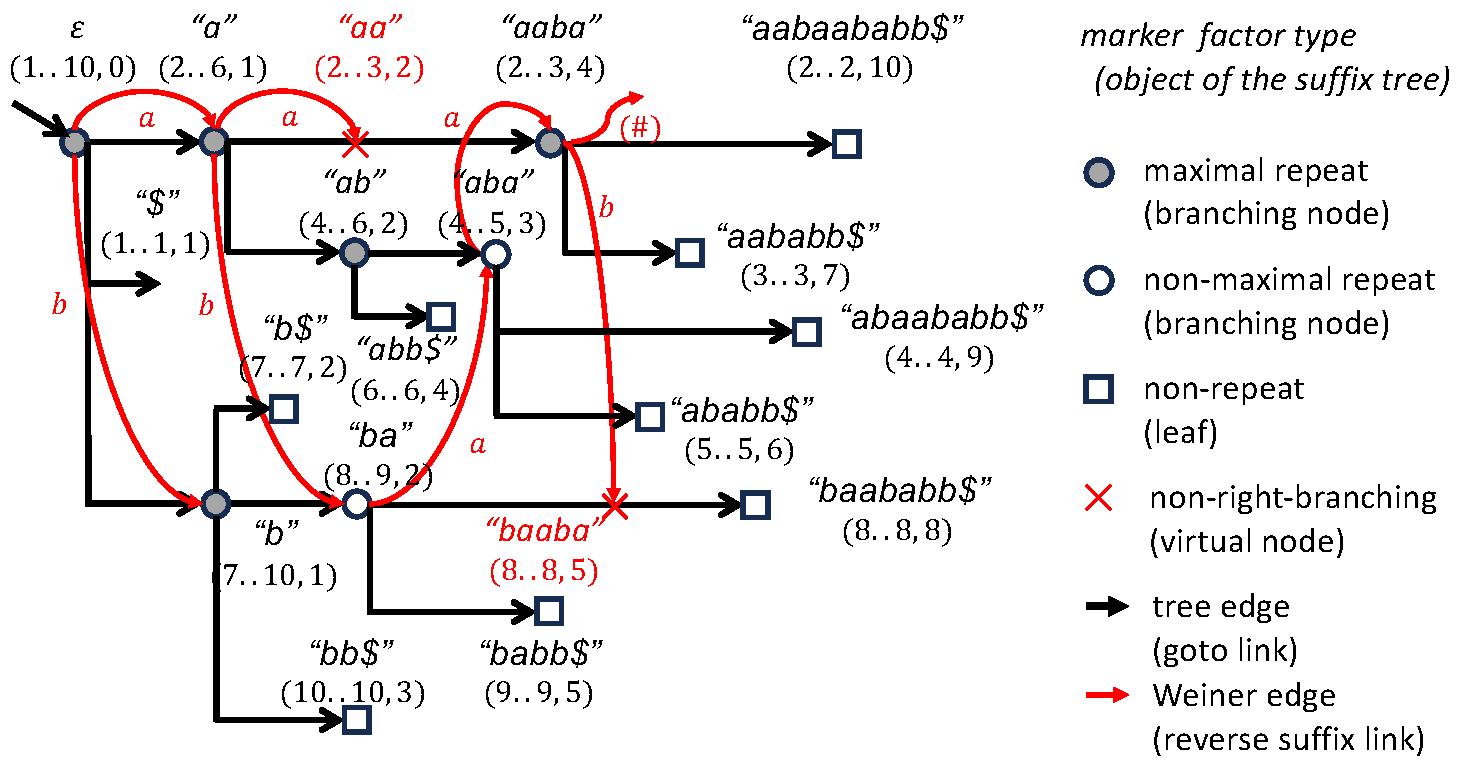
\includegraphics[width=0.9\textwidth]{fig2.pdf}
\vspace{.75\baselineskip}
\caption{An example run of Algorithm $\MREnum$ for a string $S = \mathtt{aabaababb\$}$, where the left endmarker $S[0]=\#$ and the related suffixes are omitted. 
}\label{fig:run:example}
\end{figure}
%%%%%%

%% %%%%
%% \subsection{Time-space trade-offs }
%% \label{sec:appl}

For the uncompressed SA index, the next result follows. 

\begin{theorem}\label{thm:algo:uncompressed:sa}
  The set $\MR(S)$ of all distinct maximal repeats in a string $S$ of length $n$ can be enumerated in $O(e_R)$ time and $O(\sigma^2 \log n)$ working space based on $SA, ISA, S$, and $RMQ_{LCP}$ using $O(n)$ words of space. 
\end{theorem}

\begin{proof}
%% \begin{statement}{The proof for \cref{thm:algo:uncompressed:sa}}
  From \cref{thm:algo:main} above, we obtain the next result by subsitution $t_\fn{acc}(n) = O(1)$ time and $s_\fn{acc}(n) = O(n)$ words from Manber and Myers~\cite{manber:myers1993suffixarrays}.
  \qed 
  %% \end{statement}
\end{proof}

%% \begin{trivlist}\item[] \textbf{\cref{thm:algo:uncompressed:sa}}
%%   All distinct maximal repeats in a string $S$ of length $n$ can be enumerated in $O(e_R)$ time and $O(\sigma^2 \log n)$ working space using $O(n)$ space based on $SA$, $ISA$, and the RMQ structure on $LCP$.
%% \end{trivlist}

%% \begin{theorem}\label{thm:algo:uncompressed:sa}
%%   All distinct maximal repeats in a string $S$ of length $n$ can be enumerated in $O(e_R)$ time and $O(\sigma^2 \log n)$ working space using $O(n)$ space based on $SA$, $ISA$, and the RMQ structure on $LCP$.
%% \end{theorem}


%%%%%%%%%%
%%% table2.tex : basic text indexing structures
%%%%% table2.tex

%% basic text indexing structures : array-based 
\begin{table}[t]\centering\tabcolsep=.25em
\caption{Array-based text indexing structures for static texts, where
the columns SA, ISA, TA, and LCE indicate the times for accessing the  suffix and the inverse suffix arrays, text $T$, and the LCE query. See \cref{table:summary} for $s_r(n)$  and $s_\delta(n)$. 
}\label{table:arrays}
\medskip
\begin{tabular}{l>{\centering}p{5em}>{\centering}p{7em}cccclll}\toprule
Structure	& Construct\-ion time   & Space (words) & \multicolumn{3}{c}{Query time}	\\
\cmidrule{4-6}
& &  & SA \& ISA	& TA	& LCE	 \\
  \midrule
MM~\cite{manber:myers1993suffixarrays}	& $O(n)$   & $O(n)$	& $O(1)$	& $O(1)$	& $O(1)$	\\
Belazzougui+~\cite{belazzougui2020linear} & $O(n)$   & $O(n\log n/\log\sigma)$	& $O(1)$	& $O(1)$	& $O(1)$	\\
%$s_r(n) = O(r\log(n/r)\log n)$, 
Gagie+~\cite{gagie:navarro:prezza2020fully}	& $s_r(n)$   & $O(r\log(n/r))$	& $O(\log(n/r))$	& $O(\log(n/r))$	& $O(\log(n/r))$	\\
Kempa+~\cite{kempa:kociumaka2023collapsing}	& $s_\delta(n)$   & $O(\delta \log\frac{n\log\sigma}{\delta\log n})$	& $O(\log^{4+\eps} n)$	& $O(\log n)$	& $O(\log n)$	\\
%% na	& sp	& sa	& isa	& ta	& lce	& reference \\
\bottomrule
\end{tabular}
\end{table}
%% EOF


 %% static indexes 
%% basic text indexing structures : array-based 
\begin{table}[t]\centering\tabcolsep=.25em
\caption{%%
  Array-based text indexing structures, where SA, ISA, Txt, and RMQ$_\fn{LCP}$ indicate the access and query time to the respective structures.
}\label{table:arrays:hybrid}
\medskip
\begin{tabular}{l>{\centering}p{7em}>{\centering}p{4em}cccclll}\toprule
  Structure  & Space & Constr. & \multicolumn{3}{c}{Query time}	\\
\cmidrule{4-6}
& (words) & time  & SA \& ISA	& Txt	& RMQ$_\fn{LCP}$
\\
  \midrule
Manber+~\cite{manber:myers1993suffixarrays}	& $O(n)$   & $O(n)$	& $O(1)$	& $O(1)$	& $O(1)$	\\
Ferragina+~\cite{Ferragina05:FM}  & $O(n\log n/\log\sigma)$	& $O(n)$  & $O(1)$	& ---	&
$O(1)$
%% ($O(1)$ WT)
\\
%$s_r(n) = O(r\log(n/r)\log n)$, 
%% Belazzougui+~\cite{belazzougui2020linear}  & $O(n\log n/\log\sigma)$	& $O(n)$  & $O(1)$	& $O(1)$	& $O(1)$	\\
%% %$s_r(n) = O(r\log(n/r)\log n)$, 
Gagie+~\cite{gagie:navarro:prezza2020fully}	& $O(r\log(n/r))$	& See~\cite{gagie:navarro:prezza2020fully}   & $O(\log(n/r))$	& $O(\log(n/r))$	& $O(\log(n/r))$	\\
Kempa+~\cite{kempa:kociumaka2023collapsing}	& $O(\delta \log\frac{n\log\sigma}{\delta\log n})$	& See~\cite{kempa:kociumaka2023collapsing}   & $O(\log^{4+\eps} n)$	& $O(\log n)$	& $O(\log n)$	\\
%% na	& sp	& sa	& isa	& ta	& lce	& reference \\
\bottomrule
\end{tabular}
\end{table}
%%%%%%%%%%
%% \end{toappendix}

%%% 
Next, we present the following results on the time-space trade-offs of our algorithm $\MREnum$ in \cref{thm:algo:main} by varying an underlying SA-index structure supporting $SA$, $ISA$, and $RMQ_{LCP}$.
%% \begin{toappendix}
In \cref{table:arrays:hybrid}, we show the list of underlying data structures, implementing the indexing arrays used in the following result. 


%%\cref{thm:applications}\cref{item:result:compressed:r:index}    

\begin{theorem}[Time-space trade-off]\label{thm:applications}
  We can enumerate the set $\MR(S)$
  %of all distinct maximal repeats
  in a string $S$ of length $n$ over an alphabet of $\sigma\ge 2$ symbols in the following time and space complexities, where the working space is always $O(\sigma^2 \log e_R)$. 
  %%%% 
\newcommand{\mylistheading}{\textbf}
  \begin{enumerate}[(a)]

\item \mylistheading{Bi-directional SA-index}:    
  The set $\MR(S)$ can be enumerated in $O(\min\set{e_L, e_R})$ time and $O(n)$ space using the uncompressed SA-indexes for $S$ and $S\rev$. 
  \label{item:result:bidirect:index}
    
  \item \mylistheading{$r$-sized SA-index}:
    The set $\MR(S)$  can be enumerated in $O(e_R \log {\frac n r})$ time and $O(r\log {\frac n r}\log n)$ space using the $r$-index by
    Gagie et al.~\cite{gagie:navarro:prezza2020fully}.
      \label{item:result:compressed:r:index}    
    %% Gagie et al., Navarro, and Prezza~\cite{gagie:navarro:prezza2020fully}.
    %%   \label{item:result:compressed:r:index}    
    
  \item \mylistheading{$\delta$-sized SA-index}:
    The set $\MR(S)$ can be enumerated in $O(e_R \log^{4+\eps}(n))$ time and $O(\delta\log({\frac n \delta}) \log n)$ space using the compressed SA with $\delta$-space, proposed by Kempa and Kociumaka~\cite{kempa:kociumaka2023collapsing}.
          \label{item:result:compressed:delta:index}
  \end{enumerate}
\end{theorem}

\begin{proof}
By substituting the data structures in \cref{table:arrays:hybrid} for the algorithm scheme $\MREnum$, the results immediately follows from \cref{thm:algo:main}. \qed
\end{proof}

Related to \ref{item:result:bidirect:index} of \cref{thm:applications}, Inenaga and Kosolobov~\cite{inenaga:kosolobov2024relating:left:right} recently showed that $e_R(S)$ and $e_L(S)= e_R(S\rev)$ are polynomially related with factor $\Theta(\sqrt{n})$. 
%%$\max\set{e_R(S)/e_L(S), e_L(S)/e_R(S)} = O(\sqrt{n})$. 


   %%  In this paper, we studied the problem of enumerating all distinct maximal repeats in a given string using the suffix array (SA) in relation to a repetitiveness measure $e_R$ of the number of right-extensions in a string. After examining the previous approaches, we presented a simple and efficient algorithm with novel search strategy. We proved that the proposed algorithm runs in $O(e_R)$ time based on the SA, inverse SA, and the range-minima query on the LCP array. We also show that
   %% all maximal repeats can be enumerated in $O(e_R \;\textrm{polylog}(n))$ time and space simultaneously using existing compressed text indexes. 
   %%  This is the first result on the repetitiveness-aware sublinear time algorithm for highly-repetitive strings. 


%% %%%%%%%%%%%%%%%%%
%% \begin{algorithm}[h]
%%   \caption{Enumerating all distinct maximal repeats in a string}\label{algo:maxrep:tdfw}
%%   \stringbf{Procedure} \stringsc{MaxRepTD}$(\tau = (L_0, R_0, \ell_0))$:\\
%%   %%\KwGiven{}
%%   \KwIn{The triple $\tau_0 = (L_0, R_0, \ell_0)$ for a right-branching substring $X$ of a string.}
%%   %% \KwOut{}
%%   \Begin{
%%       \stringbf{output} $\tau$
%%       \Comment*{A maximal repeat is found}
%%       %% $C \gets \emptyset$\; 
%%       %% $\stringsc{BranchRepeats}(\tau_0, C)$\; 
%%         \For (\CM{$R - L \ge 1$ must hold}) {$(L, R)\in \stringsc{BranchRepeats}(\tau_0)$}{
%%         %% \For (\CM{$R - L \ge 1$ must hold}) {$(L, R)\in C$}{
%%           $\tau \gets (L, R, \ell)$ with $\ell \gets RMQ_{LCP}(L+1, R)$
%%           \Comment*{$\tau$ is right-branching}
%%           Decide if $\tau$ is left-branching by SA and ISA (\cref{lem:leftmaximal:character})\; 
%%           \If {$\tau$ is left-branching}{          
%%             \stringsc{MaxRepTD}$(\tau)$\; 
%%           }
%%         }
%%   }
%% \end{algorithm}
%% %%%%%%%%%%%%%%%%%

